
\section{Lexicographic Fréchet Distance with Degenerate Inputs}\label{lex_frechet_deg}

\subsection{Problem}

As \citeauthor{rotelex} describes in section 7 of his paper \citetitle{rotelex} and as we hinted to in section \ref{sec:lex_frechet_alg} of this paper, multiple critical events can occur for the same $\epsilon$.

Multiple critical events for the same $\epsilon$ turn out to be problematic, because as can be seen in algorithm \ref{alg:lex_frechet_alg}, we assume the functions defined in algorithm \ref{alg:lex_frechet_alg_req} return only one critical event which then will be traversed. This assumption does not hold in all cases.

This section aims to answer the question of how to handle multiple critical events with the same critical $\epsilon$ by visualizing the problem and postulating an algorithm that decides which combination of critical events result in a lexicographic traversal. The basis of this section is section 7 of \citeauthor{rotelex}'s paper \citetitle{rotelex}\cite{rotelex}.


\subsection{Examples}

In this subsection, four examples will be discussed, for which multiple critical events for the same critical $\epsilon$ require a decision on which of them should be traversed to result in a lexicographic traversal. Instead of providing in-depth detail on solutions, this subsection aims to illustrate the problem through examples.


\subsubsection{Minimal Example: Traverse Both}\label{sec:ces_min_1}
% https://abegehr.github.io/frechet/?p=(5_5)(8_5)(2_5)(5_5)&q=(5.5_3)(4.5_7)

\begin{figure}[H]
    \centering
    
    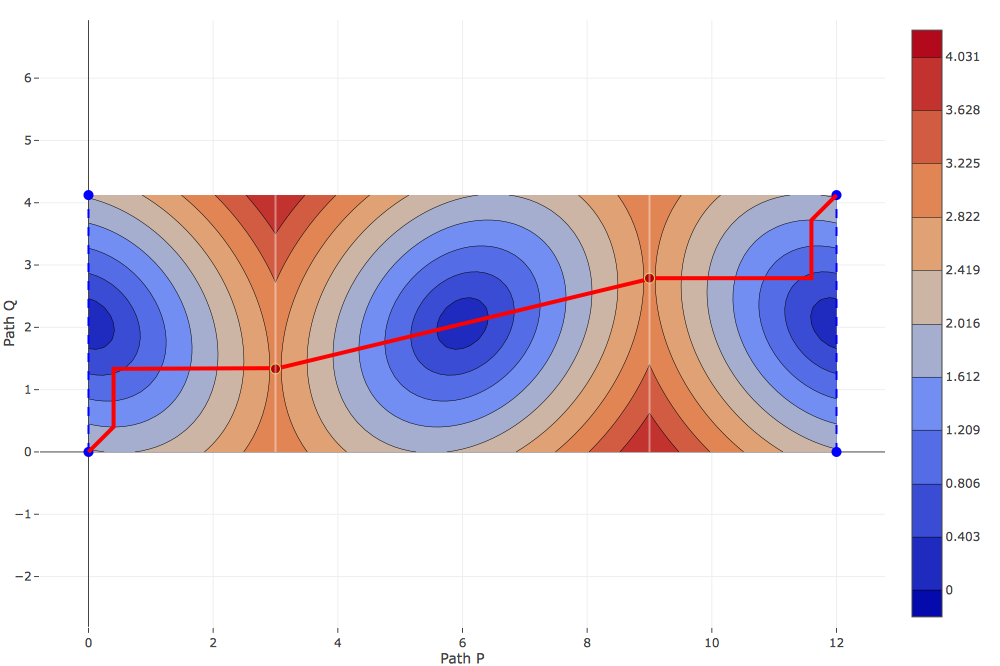
\includegraphics[width=0.8\textwidth]{ces_min_1_tra.png}
		
	\caption{One Path Over Two Critical Events\protect\footnotemark}
    \label{fig:ces_min_1}
\end{figure}
\footnotetext{View the example here: \url{https://abegehr.github.io/frechet/?p=(5_5)(8_5)(2_5)(5_5)&q=(5.5_3)(4.5_7)}}

Figure \ref{fig:ces_min_1} shows a minimal example with two critical events with the same $\epsilon$. There are two classical critical events of type b at $\epsilon \approx 2.91$ at the two vertical cell-borders. Both critical events need to be traversed.


\subsubsection{Minimal Example: Traverse Either}
% https://abegehr.github.io/frechet/?p=(4_5)(8_5)(4_5)&q=(5_4)(5_7)(5_4)

\begin{figure}[H]
    \centering
    
    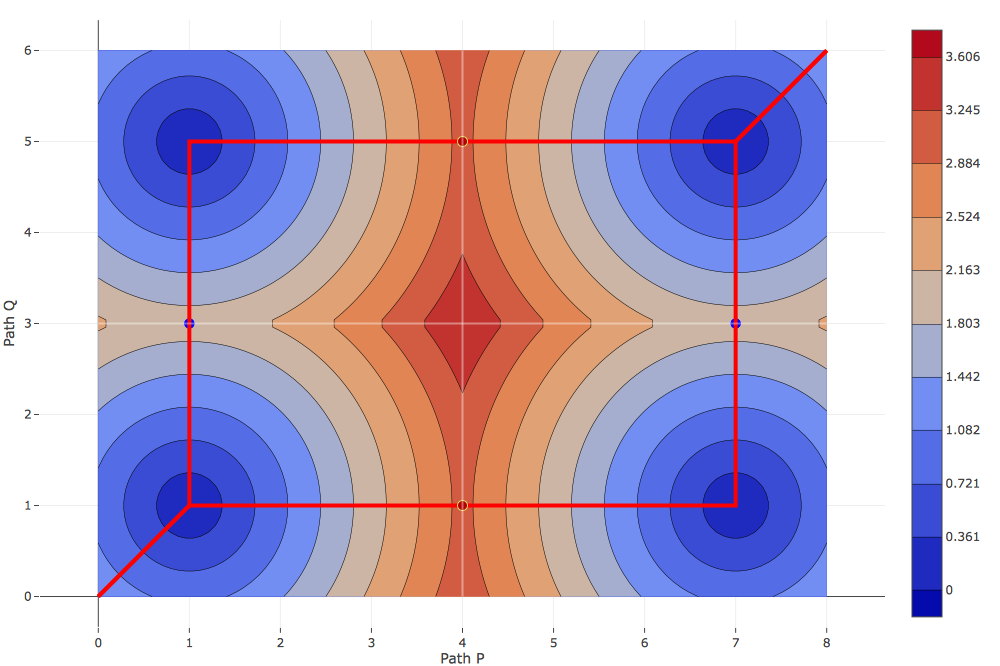
\includegraphics[width=0.8\textwidth]{ces_min_2_tra.png}
		
	\caption{Two Equivalent Paths\protect\footnotemark}
    \label{fig:ces_min_2}
\end{figure}
\footnotetext{View the example here: \url{https://abegehr.github.io/frechet/?p=(4_5)(8_5)(4_5)&q=(5_4)(5_7)(5_4)}}

Figure \ref{fig:ces_min_2} shows a minimal example of multiple critical events for the same $\epsilon$. There are four critical events to consider. Two classical critical events of type b with equal $\epsilon = 3$ at the two vertical cell-borders. And two classical critical events of type b with equal $\epsilon = 2$ at the two horizontal cell-borders. The decision problem shows that $\epsilon = 3$ is needed to traverse this height function $\delta$. Either one of the critical events at $\epsilon = 3$ needs to be traversed.



\subsubsection{Minimal Example: Traverse One}
% https://abegehr.github.io/frechet/?p=(3_2)(3_8)(6_4)&q=(2_3)(8_3)(2_3)

\begin{figure}[H]
    \centering
    
    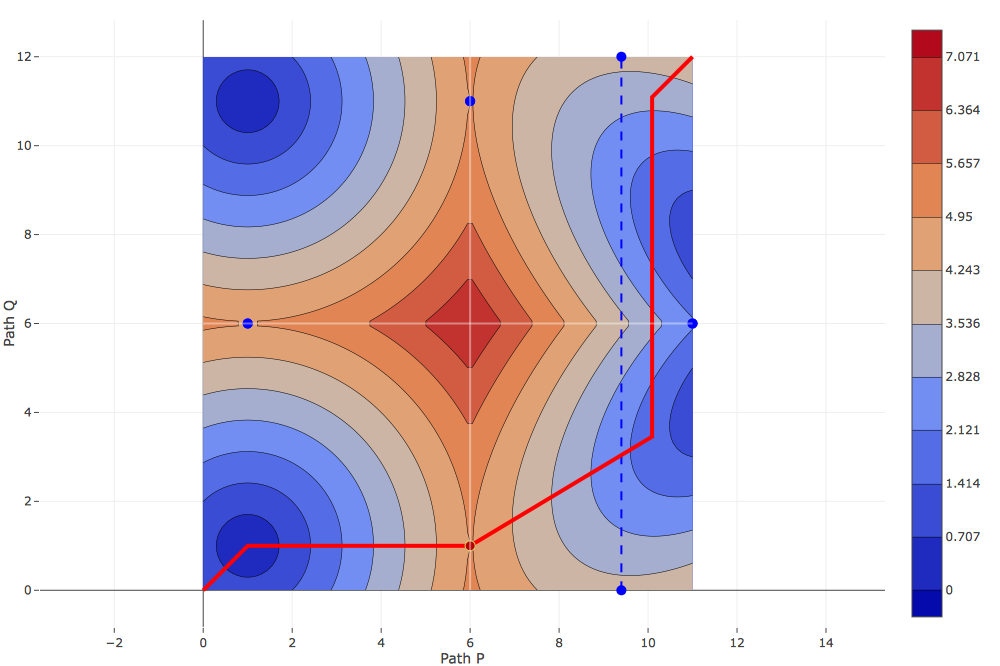
\includegraphics[width=0.8\textwidth]{ces_min_3_tra.png}
		
	\caption{Two Inequivalent Paths\protect\footnotemark}
    \label{fig:ces_min_3}
\end{figure}
\footnotetext{View the example here: \url{https://abegehr.github.io/frechet/?p=(3_2)(3_8)(6_4)&q=(2_3)(8_3)(2_3)}}

Figure \ref{fig:ces_min_3} shows three classical critical events of type b at $\epsilon = 5$ to consider: $C_1(6|1)$, $C_2(1|6)$, and $C_3(6|11)$. There are two possible paths through these three critical events: traversing just $C_1$ or traversing $C_2$ and $C_3$. Since the ascends to and descends from $C_1$, $C_2$, and $C_3$ are similar, we choose the path over only $C_1$.



\subsubsection{Complex Example}

Figure \ref{fig:ces_com} shows a more complex example of multiple critical events for the same $\epsilon$. 



\subsection{Possible Paths} \label{sec:gengraph}

We have seen in the examples that in some cases we need to traverse a path through multiple of the critical events at equal height $\epsilon_0$, while in other cases a path through one critical event is sufficient. To decide which path to traverse, first, we need to find all possible paths through the critical events.

The possible paths through multiple critical events can be represented as a graph. The start node represents the lower left corner $A$ and the end node represents the upper right corner $B$ of the current $\delta$ subsection. Each critical event $C_k \in C$ of height $\epsilon_0$ is a node. Edges are directional and denote traversability without another critical event of height $\epsilon_0$ in between.

To generate this graph, first, we use the free-space diagram represented by $L_{ij}^F$ and $B_{ij}^F$ and the decision algorithm (see \citet{altgodau}) to generate the reachable border bounds $L_{ij}^R$ and $B_{ij}^R$ of all cells. Then we use the reachable border bounds and the critical events $C$ at height $\epsilon_0$ to generate for each vertical and horizontal cell-border which subset of critical events $C$ can reach the border. We call the subset of $C$ that reaches the left and bottom border of cell $(i,j)$: $L_{ij}^C$ and $B_{ij}^C$ respectively. After computing each $L_{ij}^C$ and $B_{ij}^C$, we then connect critical events in $L_{ij}^C$ and $B_{ij}^C$ to reachable critical events starting on the top and right border.

See the algorithm \ref{alg:gengraph} for more detail on how we generate the traversability graph of multiple critical traversals $C_k$ that are at same height $\epsilon_0$. $p$ and $q$ is the number of cells between the starting-point $A$ and the ending-point $b$.


\begin{algorithm}[H]
\caption{Generate Traversability Graph of multiple critical events at $\epsilon_0$}\label{alg:gengraph}
\begin{algorithmic}[1]

\Function{GenerateTraversalGraph($A, B, C, \epsilon_0$)}{}
	\State\Comment{$A$ is start-point of traversal. $B$ is ending-point of traversal. $C$ holds all critical events $C_k$.}
	
	\State {Add $A$ and $B$ as critical events to $C$.}

	\State {$\forall i,j: L_{ij}^C := \{\} \wedge B_{ij}^C := \{\}$}
	
	\State $L^R, B^R \gets$ \Call{DecisionAlgorithm'}{$A, B, \epsilon_0$}

	\For {$C_k \in C$}
		\State {Add $C_k.B$ (ending-points) to $L_{ij}^C$ or $B_{ij}^C$ where $C_k.B$ lies.}
	\EndFor

	\For {$i := 0$ to $p$} {determine $L_{i, 0}^C$} \EndFor
	\For {$j := 0$ to $q$} {determine $B_{0,j}^C$} \EndFor
	 
	\For {$i := 0$ to $p$}
		\For {$j := 0$ to $q$}
			
			\For {$C_{k2}$ that starts on right or top border}
				\For {$C_{k1} \in L_{i, j}^C \cup B_{i, j}^C$}
					
					\If {$C_{k1}$ can reach $C_{k2}$} \label{alg:gengraph_reach}
						\State {Add edge $(C_k1$, $C_k2)$ to graph.}
					\EndIf
					
				\EndFor
			\EndFor
			
			\State {construct $L_{i+1, j}^C$ and $B_{i, j+1}^C$ from $L_{ij}^C$, $B_{ij}^C$, $L_{i+1, j}^R$, $B_{i, j+1}^R$}
		
		\EndFor
	\EndFor
	
	\Return {graph}

\EndFunction

\end{algorithmic}
\end{algorithm}

\subsubsection{Can $C_{k1}$ reach $C_{k2}$?}

In the above algorithm \ref{alg:gengraph} on line \ref{alg:gengraph_reach}, we seek to determine if the critical event $C_{k1}$ can reach the critical event $C_{k2}$. It is known that $C_{k1}$ can reach the left or bottom border of the current cell $(i, j)$, because $C_{k1} \in L_{i, j}^C \cup B_{i, j}^C$. It is also know that $C_{k2}$ starts at the top or right border of the current cell.

We discard the potential edge $(C_{k1}, C_{k2})$ in the trivial case, where $C_{k2}$ is not monotonically reachable from $C_{k1}$: $\neg(C_{k1}.B.x \leq C_{k2}.A.x \wedge C_{k1}.B.y \leq C_{k2}.A.y)$.

To determine if $C_{k2}$ is reachable from $C_{k1}$, we first look at if $C_{k1}$ comes from the left or bottom border and if $C_{k2}$ starts on the right or top border. There are four cases to consider:

\begin{enumerate}
	\item $C_{k1} \in L_{i, j}^C$ enters on left border and $C_{k2}$ starts on right border.
	\item $C_{k1} \in L_{i, j}^C$ enters on left border and $C_{k2}$ starts on top border.
	\item $C_{k1} \in B_{i, j}^C$ enters on bottom border and $C_{k2}$ starts on right border.
	\item $C_{k1} \in B_{i, j}^C$ enters on bottom border and $C_{k2}$ starts on top border.
\end{enumerate}

Reachability intervals $I_{ij}$ of right and top borders can be computed as follows:

\begin{enumerate}
	\item From left to right: $I_{ij}^{l \rightarrow r} = L_{i, j}^R \cap L_{i+1, j}^R$
	\item From left to top: If $L_{i, j}^R$ is open: $I_{ij}^{l \rightarrow t} = B_{i, j+1}^R$. Otherwise closed.
	\item From bottom to right: If $B_{i, j}^R$ is open: $I_{ij}^{b \rightarrow r} = L_{i+1, j}^R$. Otherwise closed.
	\item From bottom to top: $I_{ij}^{b \rightarrow t} = B_{i, j}^R \cap B_{i, j+1}^R$
\end{enumerate}

The superscript denotes the sides of the cell. $I_{ij}^{b \rightarrow t}$ for example represents the reachability interval of the top border for traversals coming from the bottom border.

It can be considered to use solely these reachability intervals $I_{ij}$ to decide if $C_{k2}$ can be reached from $C_{k1}$. One would simply check if $C_{k2}$ lies in the reachability intervals from the side on which $C_{k1}$ lies. This is not sufficient, as the example visualized in figure \ref{fig:gengraph_ex1} shows.

\begin{figure}[H]
    \centering
    
    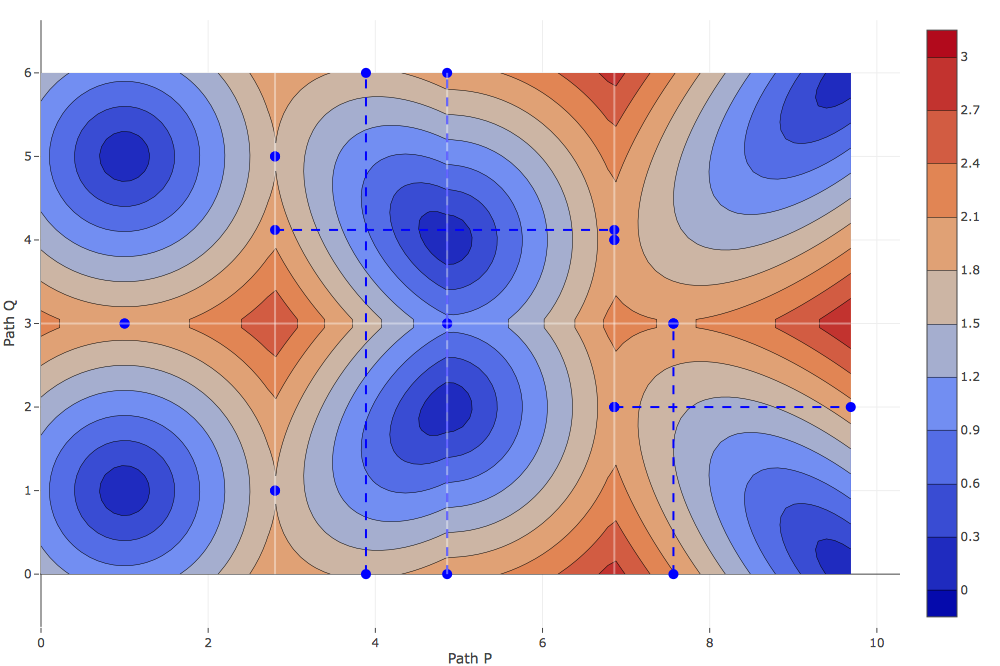
\includegraphics[width=0.8\textwidth]{gengraph_ex1.png}
		
	\caption{Considering solely reachability intervals is not sufficient\protect\footnotemark}
    \label{fig:gengraph_ex1}
\end{figure}
\footnotetext{View the example here: \url{https://abegehr.github.io/frechet/?p=(5_5)(5_7.8)(4_6)(4_8)(6_6)&q=(6_6)(3_6)(6_6)}}

In figure \ref{fig:gengraph_ex1} the decision algorithm tells us that the classical Fréchet distance is $\epsilon_F = 2$. There are two critical events of type b with $\epsilon = 2$ that we consider: $C_1(3, 1)$ and $C_2(\sim6.86, 4)$. If we were to use solely the reachability intervals to check if $C_{k2}$ is reachable from $C_{k1}$ as described above, the generated graph would find an edge between $C_1$ and $C_2$, even though there exists no such path, because it is closed by the right border of cell $(0, 1)$: $L_{1, 1}^R$. Using solely the reachability intervals, $C_2$ would still appear reachable from $C_1$, because $L_{2, 1}^R$ starts below $L_{1, 1}^R$, since $L_{2, 1}^R$ can also be reached from $B_{1,1}^R$, and not just from $L_{1, 1}^R$. We can now learn from this counter example and apply better measures.

To solve the problem of reachability intervals for generating a traversability graph of critical events, we need to memorize for each critical event not just that it can reach border $L_{ij}$ or $B_{ij}$, but also for vertical borders the minimum $y$-coordinate and for horizontal borders the minimum $x$-coordinate that it needs to reach the border, as these can differ for different critical events that both reach a border. Then, when we connect a critical event $C_{k1}$ to $C_{k2}$, we test the reachability intervals and we determine if the $C_{k2}$ lies on or above the minimum $x$- or $y$-coordinate that $C_{k1}$ needs to reach the border in question.

We can now define two helper algorithms in more detail. First, the algorithm for determining if $C_{k1}$ can reach $C_{k2}$. And second, the algorithm that constructs $L_{i+1, j}^C$ and $B_{i, j+1}^C$ from $L_{ij}^C$, $B_{ij}^C$, $L_{i+1, j}^R$, $B_{i, j+1}^R$.

\begin{algorithm}[H]
\caption{Generate Traversability Graph Helper Functions}\label{alg:gengraph_help}
\begin{algorithmic}[1]

\Function{CanReach($C_{k1}, min_{x}, min_{y}, C_{k2}, I_{ij}^{l \rightarrow r}, I_{ij}^{l \rightarrow t}, I_{ij}^{b \rightarrow r}, I_{ij}^{b \rightarrow t}$)}{}
	\State\Comment{Determines if $C_{k1}$ can reach $C_{k2}$.}
	
	\If {$C_{k1}$ is on left border and $C_{k2}$ is on right border}
		\State\Return {$C_{k2}.A.y \in I_{ij}^{l \rightarrow r} \wedge C_{k2}.A.y \geq min_{y}$}
	\EndIf
	\If {$C_{k1}$ is on left border and $C_{k2}$ is on top border}
		\State\Return {$C_{k2}.A.x \in I_{ij}^{l \rightarrow t} \wedge C_{k2}.A.x \geq min_{x}$}
	\EndIf
	\If {$C_{k1}$ is on bottom border and $C_{k2}$ is on right border}
		\State\Return {$C_{k2}.A.y \in I_{ij}^{b \rightarrow r} \wedge C_{k2}.A.y \geq min_{y}$}
	\EndIf
	\If {$C_{k1}$ is on bottom border and $C_{k2}$ is on top border}
		\State\Return {$C_{k2}.A.x \in I_{ij}^{b \rightarrow t} \wedge C_{k2}.A.x \geq min_{x}$}
	\EndIf
\EndFunction

\State

\Function{ConstructCriticalReach($L_{ij}^C$, $B_{ij}^C$, $L_{i+1, j}^R$, $B_{i, j+1}^R$)}{}
	\State\Comment{Constructs $L_{i+1, j}^C$ and $B_{i, j+1}^C$ from $L_{ij}^C$, $B_{ij}^C$, $L_{i+1, j}^R$, $B_{i, j+1}^R$}
	
	\State {$L_{i+1, j}^C := \{\}$}
	\State {$B_{i, j+1}^C := \{\}$}
	
	\If {$L_{i+1, j}^R$ is not closed}
		\For {$(C_k, min_{x}) \in B_{ij}^C$}
			\State {Add $(C_k, L_{i+1, j}^R.min)$ to $L_{i+1, j}^C$}
		\EndFor
		\For {$(C_k, min_{y}) \in L_{ij}^C$}
			\If {$min_{y} \leq L_{i+1, j}^R.max$}
				\State {$min_{y} \gets max(min_{y}, L_{i+1, j}^R.min$)}
				\State {Add $(C_k, min_{y})$ to $L_{i+1, j}^C$}
			\EndIf
		\EndFor
	\EndIf
	
	\If {$B_{i, j+1}^R$ is not closed}
		\For {$(C_k, min_{y}) \in L_{ij}^C$}
			\State {Add $(C_k, B_{i, j+1}^R.min)$ to $B_{i, j+1}^C$}
		\EndFor
		\For {$(C_k, min_{x}) \in B_{ij}^C$}
			\If {$min_{x} \leq B_{i, j+1}^R.max$}
				\State {$min_{x} \gets max(min_{x}, B_{i, j+1}^R.min$)}
				\State {Add $(C_k, min_{x})$ to $B_{i, j+1}^C$}
			\EndIf
		\EndFor
	\EndIf
	
	\State\Return {$L_{i+1, j}^C, B_{i, j+1}^C$}
	
\EndFunction

\end{algorithmic}
\end{algorithm}

The two functions defined in algorithm \ref{alg:gengraph_help} are necessary for algorithm \ref{alg:gengraph} to generate the correct traversability graph for a set of critical events at the same height $\epsilon_0$.

Checking if $C_{k2}.A$ lies in the respective reachability interval might be superfluous, because we are already checking for the minimum $x$- or $y$-coordinate. Nevertheless, also checking the reachability interval $I_{ij}$ does not hurt the valid functioning.


\subsection{Traversal cross-section $f(t)$ and profile $\hat{f}(s)$}\label{sec:trav_csp}

In this section we will define a traversals cross-section $f(t)$ and its profile $\hat{f}(s)$.

\subsubsection{Hyperbolas}

Due to our input being two paths consisting of connected straight line-segments, every straight cross-section through our height function $\delta$ is a continuous composition of hyperbolas. We use the following function to denote these hyperbolas $h$:

$$h: \epsilon(t) = \sqrt{u^2 + a(t - v)^2}$$

Each hyperbola has three parameters $u$, $a$, and $v$. A hyperbola is always a cross-section though a segment of the height function $\delta$. An equation system is used to determine the three parameters $u$, $a$, and $v$. There are two cases to consider:

\begin{enumerate}
	\item For a horizontal of vertical cross-section, $a = 1$. Therefore, only two points $(t, \epsilon)$ are needed to determine $u$ and $v$. The two points $(t, \epsilon)$ are calculated by sampling two pairs of points from the input line-segments and determining there $t$ and distance $\epsilon$.
	\item For a diagonal cross-section three points $(t, \epsilon)$ are needed to determine $u$, $a$ and $v$. The two points $(t, \epsilon)$ are calculated by sampling three pairs of points from the input line-segments and determining there $t$ and distance $\epsilon$.
\end{enumerate}

For simplicity, we define the hyperbolas all as starting at $t=0$. This can be done by adjusting the parameter $v$.


\subsubsection{Cross-Section $f(t)$}

To attain a cross-section $f(t)$ of an entire traversal, we simply create a composite function of the $N$ hyperbolas and move them along the $t$-axis to the correct position. This yields $f(t)$. $t_k$ is the time interval in which the $k^{th}$ hyperbola is traversed.

\[ f(t) =
\begin{cases} 
	\sqrt{u_1^2 + a_1(t - v_1)^2} & 0 \leq t \leq t_1 \\
	\sqrt{u_2^2 + a_2(t - v_2 - t_1)^2} & t_1 \leq t \leq t_2 \\
	\dots \\
	\sqrt{u_N^2 + a_N(t - v_N - t_{N-1})^2} & t_{N-1} \leq t \leq t_N \\
\end{cases}
\]

For the example in figure \ref{fig:ces_min_1}, the cross-section $f(t)$ is shown in figure \ref{fig:ces_min_1_cs}. The $x$-axis shows the time and the $y$-axis shows the current $\epsilon$. Notice that when the traversal moves on the $l$-lines the cross-section is linear. This is because the addend $u^2$ inside the square root equals zero for this case. Therefore, the square and the square root cancel and we are left with the absolute value of a linear function: $\left| \sqrt{a}(t - v) \right|$.

 \begin{figure}[H]
    \centering
    
    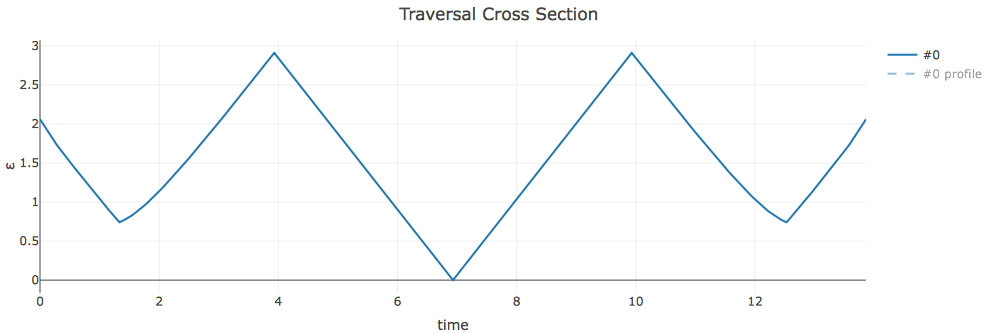
\includegraphics[width=0.8\textwidth]{ces_min_1_cs.png}
		
	\caption{Cross-section $f(t)$ for example from section \ref{sec:ces_min_1}\protect\footnotemark}
    \label{fig:ces_min_1_cs}
\end{figure}
\footnotetext{View the example here: \url{https://abegehr.github.io/frechet/?p=(4_5)(8_5)(4_5)&q=(5_4)(5_7)(5_4)}\label{ftn:ces_min_1}}


\subsubsection{Profile $\hat{f}$}

In addition to the cross-section $f(t)$, we can also look at the profile $\hat{f}(s)$. \citeauthor{rotelex} defines the profile function $\hat{f}(s)$ as the time that $\epsilon$ exceeds a threshold $s$:

$$\hat{f}(s) = \mu(\left\{ t \mid f(t) \geq s \right\})$$

where $\mu$ denotes the Lebesgue measure.\cite{rotelex}

Figure \ref{fig:ces_min_1_csp} shows the profile function $\hat{f}(s)$ in addition to the function of the cross-section shown in figure \ref{fig:ces_min_1_cs} for the example from figure \ref{fig:ces_min_1}.

 \begin{figure}[H]
    \centering
    
    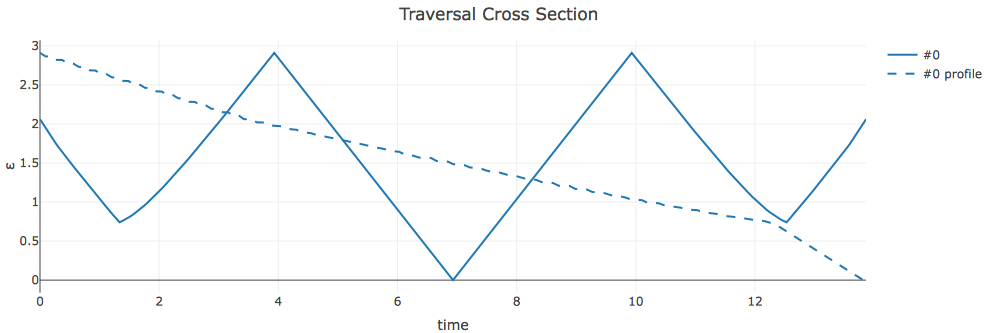
\includegraphics[width=0.8\textwidth]{ces_min_1_csp.png}
		
	\caption{Cross-section $f(t)$ and profile $\hat{f}(s)$ for example from section \ref{sec:ces_min_1}\textsuperscript{\ref{ftn:ces_min_1}}}
    \label{fig:ces_min_1_csp}
\end{figure}

The profile function $\hat{f}(s)$ is defined using the cross-section hyperbolas. It is important to note that each hyperbola function $h_j(t)$ is defined so that $0 \leq t \leq t_j - t_{j-1}$; therefore, we can simply sum up the inverses of the hyperbolas in these bounds to calculate the profile in the following two steps:

\begin{enumerate}
	\item Compute the inverse function of a hyperbolas function $h^{-1}(\epsilon)$. First solve $\epsilon(t)$ for $t$:
	
	\begin{align*}
		\epsilon & = \sqrt{u^2 + a(t - v)^2}\\
		\epsilon^2 & = u^2 + a(t - v)^2\\
		\epsilon^2 - u^2 & = a(t - v)^2\\
		\frac{\epsilon^2 - u^2}{a} & = (t - v)^2\\
		\pm\sqrt{\frac{\epsilon^2 - u^2}{a}} & = t - v\\
		v \pm \sqrt{\frac{\epsilon^2 - u^2}{a}} & = t\\
	\end{align*}
	
	This results in the following definition for $h^{-1}(\epsilon)$:
	
	\begin{align}
		h_j^{-1}: t_j(\epsilon) = 
		\begin{cases}
   			{v_j \pm \sqrt{\frac{\epsilon^2 - u_j^2}{a_j}}}	& \text{if } {h_j(0) \leq \epsilon \leq h_j(t_j - t_{j-1})}\\
   			0        										& \text{otherwise}
  		\end{cases} \label{eq:hinv}
  	\end{align}
	
	Note that $h_j$ is valid in the interval $0 \leq t \leq t_j - t_{j-1}$; therefore, $h_j^{-1}$ is defined for $h_j(0) \leq \epsilon \leq h_j(t_j - t_{j-1})$. This is important to yield the correct profile function $\hat{f}(s)$. Also notice that each hyperbola $h_j$ has its own three parameters: $u_j$, $a_j$, and $v_j$.
	
	\item Sum up the inverses to yield the profile function $\hat{f}(s)$.
	
	$$\hat{f}(s) = \sum_{j=0}^N {h_j^{-1}(s)}$$
	
\end{enumerate} 

Now we have defined the profile function $\hat{f}(s)$ for a traversal with cross-section $f(t)$ that allows us to calculate the amount of time a traverser traversing this traversal spends above the threshold $s$.

\subsection{Multiple Ascents to and Descents from $\epsilon_0$}

To fulfill our goal of a lexicographic traversal, we want to minimize the time during which the height $\epsilon$ exceeds a threshold $s$.\cite{rotelex} Concerning our examples, we want to minimize the time needed to ascend to and descend from our critical height $\epsilon_0$.

If we have multiple critical events at the critical height $\epsilon_0$, we need to decide which to choose while fulfilling our goal of a lexicographic traversal. The profile function $\hat{f}(s)$, introduced in section \ref{sec:trav_csp}, defines the time that a traversals exceeds a threshold $s$. Our goal of a lexicographic traversal is to minimize this time. This means that for two profile functions $\hat{f}(s)$ and $\hat{g}(s)$ that both are critical at $\epsilon_0$, we need to compare the derivatives.

$$\hat{f'}(s) = \left[ \sum_{j=0}^N {h_j^{-1}(s)} \right]'$$

Because of the sum rule, we can apply the derivative to each $h_j^{-1}$.

$$\hat{f'}(s) = \sum_{j=0}^N {[h_j^{-1}]'(s)}$$


\subsubsection{Simplifications and First Derivative}\label{sec:first_derivative}

Due to the form of $h_j^{-1}$ (see equation \ref{eq:hinv}), the derivative of $h_j^{-1}$ is not trivial. $h_j^{-1}$ is a composite function and has a $\pm$. We circumvent this problem by only looking at hyperbolas that ascend to and descend from the critical height $\epsilon_0$.

For a critical event $C_k$ at $\epsilon_0$, we will denote the ascent hyperbola with $h_{k\uparrow}$ and the descent hyperbola with $h_{k\downarrow}$.

We will only consider critical events with one ascent and one descent hyperbola, analogous to classical critical events of type b. Classical critical events of type c can easily be modeled by multiple critical events of type b. Classical critical events of type a and new type of lexicographic critical events consist of only one ascent or descent hyperbola.

Because of simplicity we move the hyperbolas so that $t = 0$ for the critical height $\epsilon$: $h(0) = \epsilon_0$.

The hyperbolas are vertically symmetric at $t_v=v$, $h(t_v+t) = h(t_v-t)$; therefore, the inverse hyperbolas are horizontally symmetric at $t_v = v$. This means that to get rid of the $\pm$ in the inverse and get only positive slopes, we can simply use a $+$ when we calculate the derivative:

\begin{align}
	[h^{-1}]'(\epsilon)  &= \left[ v + \sqrt{\frac{\epsilon^2 - u^2}{a}} \right]'\nonumber\\
	[h^{-1}]'(\epsilon) &= \left[\sqrt{\frac{\epsilon^2 - u^2}{a}} \right]'\nonumber\\
	[h^{-1}]'(\epsilon) &= \frac{ \left[ \frac{\epsilon^2 - u^2}{a} \right]' }{ 2\sqrt{\frac{\epsilon^2 - u^2}{a}} }\nonumber\\
	[h^{-1}]'(\epsilon) &= \frac{ \left[ \epsilon^2 - u^2 \right]' }{ 2a\sqrt{\frac{\epsilon^2 - u^2}{a}} }\nonumber\\
	[h^{-1}]'(\epsilon) &= \frac{ 2\epsilon }{ 2a\sqrt{\frac{\epsilon^2 - u^2}{a}} }\nonumber\\
	[h^{-1}]'(\epsilon)  &= \frac{ \epsilon }{ a\sqrt{\frac{\epsilon^2 - u^2}{a}} }\label{eq:hinvd1}
\end{align}

The hyperbolas are defined so that: $h(0) = \epsilon_0$; therefore, $h^{-1}(\epsilon_0) = 0$.

\begin{align}
	h^{-1}(\epsilon_0) &= v \pm \sqrt{\frac{\epsilon_0^2 - u^2}{a}}\nonumber\\
	0 &= v \pm \sqrt{\frac{\epsilon_0^2 - u^2}{a}}\nonumber\\
	-v &= \pm \sqrt{\frac{\epsilon_0^2 - u^2}{a}}\nonumber\\
	\left| -v \right| &= \left| \pm \sqrt{\frac{\epsilon_0^2 - u^2}{a}} \right|\nonumber\\
	\left| v \right| &= \sqrt{\frac{\epsilon_0^2 - u^2}{a}} \label{eq:veps0}
\end{align}

We can write a simple equation for $[h^{-1}]'(\epsilon_0)$ by using the equations \ref{eq:hinvd1} and \ref{eq:veps0}:

\begin{align}
	[h^{-1}]'(\epsilon_0)  &= \frac{ \epsilon_0 }{ a\sqrt{\frac{\epsilon_0^2 - u^2}{a}} }\nonumber\\
	[h^{-1}]'(\epsilon_0)  &= \frac{ \epsilon_0 }{ a \left| v \right| }\label{eq:hinvd1eps0}
\end{align}

Having an equation for $[h^{-1}]'(\epsilon_0)$, we will now determine the slope at $\hat{f}_{\epsilon_0}(\epsilon_0)$ by adding the ascending and descending slopes of all critical events $C$ at critical height $\epsilon_0$:

\begin{align*}
	\hat{f}'_{\epsilon_0}(\epsilon_0) &= \sum_{C_k \in C(\epsilon_0)} { [h_{k\downarrow}^{-1}]'(\epsilon_0) + [h_{k\uparrow}^{-1}]'(\epsilon_0)}\\
	\hat{f}'_{\epsilon_0}(\epsilon_0) &= \sum_{C_k \in C(\epsilon_0)} { \frac{\epsilon_0}{a_{k\downarrow} \left| v_{k\downarrow} \right|} + \frac{\epsilon_0}{a_{k\uparrow} \left| v_{k\uparrow} \right|}}
\end{align*}

There are three cases to consider:

\begin{enumerate}
	\item $\hat{f}'_{\epsilon_0}(\epsilon_0) > \hat{g}'_{\epsilon_0}(\epsilon_0)$: Choose traversal for $f$.
	\item $\hat{f}'_{\epsilon_0}(\epsilon_0) < \hat{g}'_{\epsilon_0}(\epsilon_0)$: Choose traversal for $g$.
	\item $\hat{f}'_{\epsilon_0}(\epsilon_0) = \hat{g}'_{\epsilon_0}(\epsilon_0)$: Cannot decide.
\end{enumerate}

Cases one and two are clear. Case three on the other hand, when the slope of both profiles at $\epsilon_0$ is the same, no decision can be made at that point. We would have to look at further derivatives.


\subsubsection{Second Derivative}

The the calculation of $h^{-1}$'s the second derivative:

\begin{align}
	[h^{-1}]''(\epsilon)  &= \left[ \frac{ \epsilon }{ a\sqrt{\frac{\epsilon^2 - u^2}{a}} } \right]'\nonumber\\
	[h^{-1}]''(\epsilon)  &= \frac {\left[ \frac{ \epsilon }{ \sqrt{\frac{\epsilon^2 - u^2}{a}} } \right]'}{ a }\nonumber\\
	[h^{-1}]''(\epsilon)  &= \frac { \frac{ \left[ \epsilon \right]' }{ \sqrt{\frac{\epsilon^2 - u^2}{a}} } + \epsilon \left[ \frac{1}{ \sqrt{\frac{\epsilon^2 - u^2}{a}} } \right]' }{ a }\nonumber\\
	[h^{-1}]''(\epsilon)  &= \frac { \frac{1}{ \sqrt{\frac{\epsilon^2 - u^2}{a}}}  - \frac{\epsilon \left[ \frac{\epsilon^2 - u^2}{a} \right]' }{ 2\left(\frac{\epsilon^2 - u^2}{a}\right)^{\frac{3}{2}} } }{a}\nonumber\\
	[h^{-1}]''(\epsilon)  &= \frac { \frac{1}{ \sqrt{\frac{\epsilon^2 - u^2}{a}}}  - \frac{2\epsilon^2 }{ 2a\left(\frac{\epsilon^2 - u^2}{a}\right)^{\frac{3}{2}} } }{a}\nonumber\\
	[h^{-1}]''(\epsilon)  &= \frac{1}{ a\sqrt{\frac{\epsilon^2 - u^2}{a}}}  - \frac{\epsilon^2 }{ a^2\left(\frac{\epsilon^2 - u^2}{a}\right)^{\frac{3}{2}} }\nonumber\\
	[h^{-1}]''(\epsilon)  &= \left( \frac{1}{ a\left(\frac{\epsilon^2 - u^2}{a}\right)^{\frac{1}{2}}} - \frac{\epsilon^2 }{ a^2\left(\frac{\epsilon^2 - u^2}{a}\right)^{\frac{3}{2}} } \right) \frac{\left(\frac{\epsilon^2 - u^2}{a}\right)^{\frac{3}{2}}}{\left(\frac{\epsilon^2 - u^2}{a}\right)^{\frac{3}{2}}}\nonumber\\
	[h^{-1}]''(\epsilon)  &= \left( \frac{ \epsilon^2 - u^2 }{a^2}  - \frac{\epsilon^2 }{a^2} \right) \frac{1}{\left(\frac{\epsilon^2 - u^2}{a}\right)^{\frac{3}{2}}}\nonumber\\
	[h^{-1}]''(\epsilon)  &= \left( \frac{-u^2}{a^2} \right) \frac{1}{\left(\frac{\epsilon^2 - u^2}{a}\right)^{\frac{3}{2}}}\nonumber\\
	[h^{-1}]''(\epsilon)  &= - \frac{u^2}{a^2\left(\frac{\epsilon^2 - u^2}{a}\right)^{\frac{3}{2}}}\label{eq:hinvd2}
\end{align}

We can write a simple equation for $[h^{-1}]'(\epsilon_0)$ by using the equations \ref{eq:hinvd2} and \ref{eq:veps0}:

\begin{align}
	[h^{-1}]''(\epsilon_0)  &= - \frac{u^2}{a^2 \left| v \right|^3}\label{eq:hinvd2eps0}
\end{align}

Again, we sum up all $[h^{-1}]''(\epsilon_0)$ and compare the sums of each traversal analogous to the description in section \ref{sec:first_derivative}. We choose the traversal with the larger $\sum\nolimits_{C_k \in C(\epsilon_0)}[h_{k\uparrow}^{-1}]''(\epsilon_0) + [h_{k\downarrow}^{-1}]''(\epsilon_0)$.

\subsubsection{Example: First Derivative}

Let us consider an example where we can decide from looking at the first derivative which traversal path to choose. Figure \ref{fig:ces_ad_1} shows such an example.

 \begin{figure}[H]
    \centering
    
    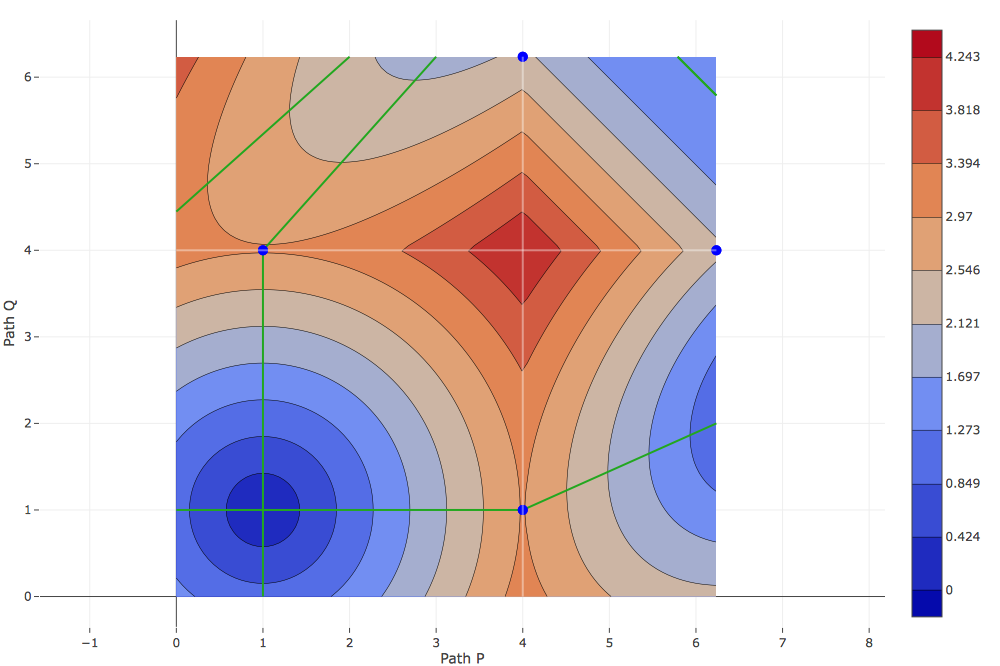
\includegraphics[width=0.8\textwidth]{ces_ad_1.png}
		
	\caption{Two critical events with unequal first derivative of profiles\protect\footnotemark}
    \label{fig:ces_ad_1}
\end{figure}
\footnotetext{View the example here: \url{https://abegehr.github.io/frechet/?p=(0_1)(4_1)(2_2)&q=(1_0)(1_4)(3_3)}}

In the example depicted in figure \ref{fig:ces_ad_1}, there are two classical critical events of type b at critical height $\epsilon_0 = 3$ to consider: $C_1(1, 4)$ and $C_2(4, 1)$.

The algorithm \ref{alg:gengraph} that generates a traversability graph for multiple critical events at the same height as defined in \ref{sec:gengraph} returns that there are two possible paths through the critical events $C_1$ and $C_2$. Either the graph is traversed from the starting-point to the ending-point over $C_1$, this will be path $f$, or over $C_2$, that will be path $g$.

We will now look at the ascent to and descent from hyperbolas of $C_1$ and $C_2$.


\begin{align*}
	h_{f1\uparrow}(t) &= \sqrt{0^2 + 1\cdot(t - (-3))^2} = \left| t + 3 \right|\\
	h_{f1\downarrow}(t) &= \sqrt{0^2 + 0.8\cdot(t - 3.354)^2} = \left| \sqrt{0.8}(t - 3.354) \right|\\
	h_{g1\uparrow}(t) &= \sqrt{0^2 + 1\cdot(t - (-3))^2} = \left| t + 3 \right|\\
	h_{g1\downarrow}(t) &= \sqrt{0^2 + 0.2\cdot(t - 6.708)^2} = \left| \sqrt{0.2}(t - 6.708) \right|
\end{align*}

Next, we calculate the specific slopes of the inverse hyperbolas at $\epsilon_0 = 3$ by using equation \ref{eq:hinvd1eps0}.

\begin{align*}
	h_{f1\uparrow}'(\epsilon_0) &= \frac{3}{1\cdot\left|-3\right|} = 1\\
	h_{f1\downarrow}'(\epsilon_0) &= \frac{3}{0.8\cdot\left|3.354\right|} \approx 1.118\\
	h_{g1\uparrow}'(\epsilon_0) &= \frac{3}{1\cdot\left|-3\right|} = 1\\
	h_{g1\downarrow}'(\epsilon_0) &= \frac{3}{0.2\cdot\left|6.708\right|} \approx 2.236 
\end{align*}

From the slopes, $\hat{f}'_{\epsilon_0}(\epsilon_0)$ and $\hat{g}'_{\epsilon_0}(\epsilon_0)$ can now be calculate:

\begin{align*}
	\hat{f}'_{\epsilon_0}(\epsilon_0) &= h_{f1\uparrow}'(\epsilon_0) + h_{f1\downarrow}'(\epsilon_0) \approx 2.118\\
	\hat{g}'_{\epsilon_0}(\epsilon_0) &= h_{g1\uparrow}'(\epsilon_0) + h_{g1\downarrow}'(\epsilon_0) \approx 3.236\\
\end{align*}

!!!TODO: g for the win!!!


\subsection{Postulate Algorithm}
Postulate algorithm for choosing a critical event from several with equal epsilon: (visual examples!)

Algorithm:
\begin{enumerate}
	\item For every critical event compute reciprocal of derivates descents and store as critical event's steepness.
	\item From set of critical events, generate all possible sequences (ascending monotone).
	\item For all sequences sum steepness of their critical events and store as sequence rank.
	\item Starting with the smallest-rank sequence, decide if the sequence of critical events is traversable without passing critical events excluded in the sequence.
	\item If decision is negative, repeat 4.
	\item If decision is positive, repeat 4 for all sequences of equal rank.
	\item If multiple sequences of equal rank are found to be valid, traverse all, and decide by comparing.
	\item The steepness of the steepest decent.
	\item The steepness of critical event that is reached.
	\item And choose the path with the steepest summed recents of all paths.
	\item If multiple paths with same hight profile are found, return all. Otherwise return the lexicographic optimum.
	\item 
\end{enumerate}

\subsection{Traversing critical events}

Assume we are traversing a heat map generated by two curves. We arrive at a point where we have to decide which critical events need to be traversed for a lexicographic solution. The decision algorithm\cite{altgodau} can be applied for the $\epsilon$ of each possible critical event. We pick the smallest $\epsilon$ for which the decision algorithm returns a positive decision. We call it $\epsilon_0$. Now two options are feasible:

\begin{enumerate}[label=(\Alph*)]
	\item There is one critical event at height $\epsilon_0$. $|C_{\epsilon_0}| = 1$
	\item There are multiple critical events at height $\epsilon_0$. $|C_{\epsilon_0}| > 1$
\end{enumerate}

In case option A holds true, this critical event will need to be traversed. The traversal-problem is divided into two sub problems, which are both examined recursively and independently.

In case option B holds true, we need to decide which of the critical events $C_{\epsilon_0}$ need to be traversed and which are not needed for an optimal solution. We will consider all subsets $C'_{\epsilon_0}$ of $C_{\epsilon_0}$ with size $n>0$.


\subsection{Example of Algorithm visualized (visual example!)}

\subsection{Analysing postulated algorithm for handling degenerate inputs}
\subsubsection{Runtime analysis}
\subsection{Real world application}
	Can you think of one?
	
	
	
